\documentclass{beamer}
\usetheme{Goettingen}
\setbeamertemplate{footline}[frame number]

\usepackage{amsmath}
\usepackage{fontspec}
\usepackage{unicode-math}
\usepackage{graphicx}
\usepackage{enumitem}
\usepackage{calc}
\usepackage{ragged2e}
\usepackage{caption}

% --- TikZ ---
\usepackage{adjustbox}
\usepackage{tikz}

\usetikzlibrary{
  math,
  shapes,
  arrows,
  arrows.meta,
  decorations.markings,
  positioning,
  fit
}

\tikzstyle{terminator} = [
  rectangle,
  draw,
  text centered,
  rounded corners,
  minimum height=2em
]

\tikzstyle{data} = [
  trapezium,
  draw,
  text centered,
  trapezium left angle=60,
  trapezium right angle=120,
  minimum height=2em
]

\tikzstyle{team} = [rectangle, draw, text centered, minimum height=2em]

\tikzstyle{connector} = [draw, -latex']

\tikzset{
  ->-/.style={
    decoration={
      markings,
      mark=at position #1 with {\arrow{>}}
    },
    postaction={decorate}
  }
}

% --- Listings ---
\usepackage{listings}

\lstset{
  language     = Python,
  basicstyle   = \ttfamily\footnotesize,
  keywordstyle = \color{magenta},
  commentstyle = \itshape\color{blue},
  stringstyle  = \color{blue},
  morekeywords = {self}
}

\lstdefinelanguage{TOML}{
  sensitive   = true,
  morecomment = [l]{\#},
  morestring  = [b]",
  morestring  = [b]',
  alsoletter  = {-},
  moredelim   = [s][\color{blue}]{[}{]}
}

% --- Hyperlinks ---
\usepackage{hyperref}

\hypersetup{
  colorlinks  = true,
  linkcolor   = blue,
  filecolor   = magenta,
  urlcolor    = cyan,
  pdftitle    = {Rocket Calculator},
  pdfpagemode = FullScreen
}

% --- Fonts ---
\setmainfont{DejaVu Sans Mono}
\setmathfont{Concrete Math}
\setmonofont{Iosevka}

%\setlist[itemize]{label=--}

\newcommand{\diff}[1]{\ensuremath{\mathop{}\!\mathrm{d}}#1}
\newcommand{\ndiff}[2]{\ensuremath{\mathop{}\!\mathrm{d}^{#1}}#2}

\title{BEARS Rocket Solver (Semi-Final)}
\subtitle{A Sufficiently General Rocket Calculator}
\date{\today}

\begin{document}

\begin{frame}
  \titlepage
\end{frame}

\begin{frame}{Outline}
  \tableofcontents
\end{frame}

\section{OpenMDAO Framework}
\begin{frame}{Hybrid rocket engine structure}
  \centering
  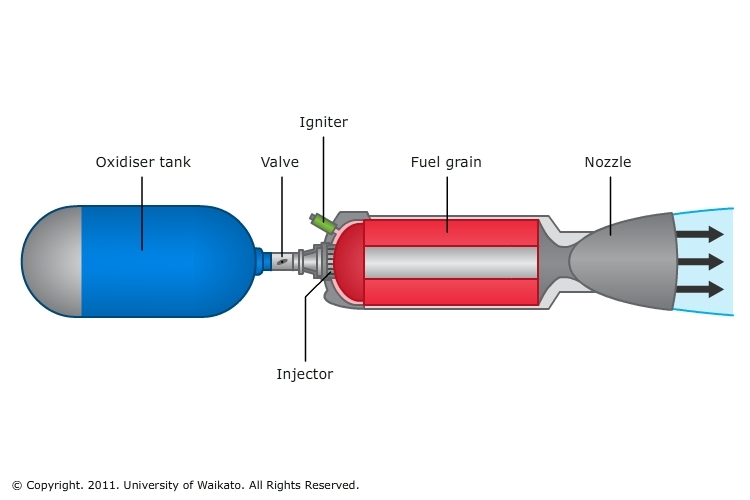
\includegraphics[width=\columnwidth]{figures/Hybrid-rocket-engine.jpg}
\end{frame}

\begin{frame}{Calculations program requirements}
  \begin{itemize}
  \item[--] \emph{Readable:} more than one person needs to be able to understand
    it
  \item[--] \emph{Extensible:} working groups should be able to extend their
    parts without impacting the rest of the assembly
  \item[--] \emph{General:} not committing to a particular design
  \end{itemize}
\end{frame}

\begin{frame}{OpenMDAO framework}
  \center{
    Solution: \textbf{OpenMDAO!}

    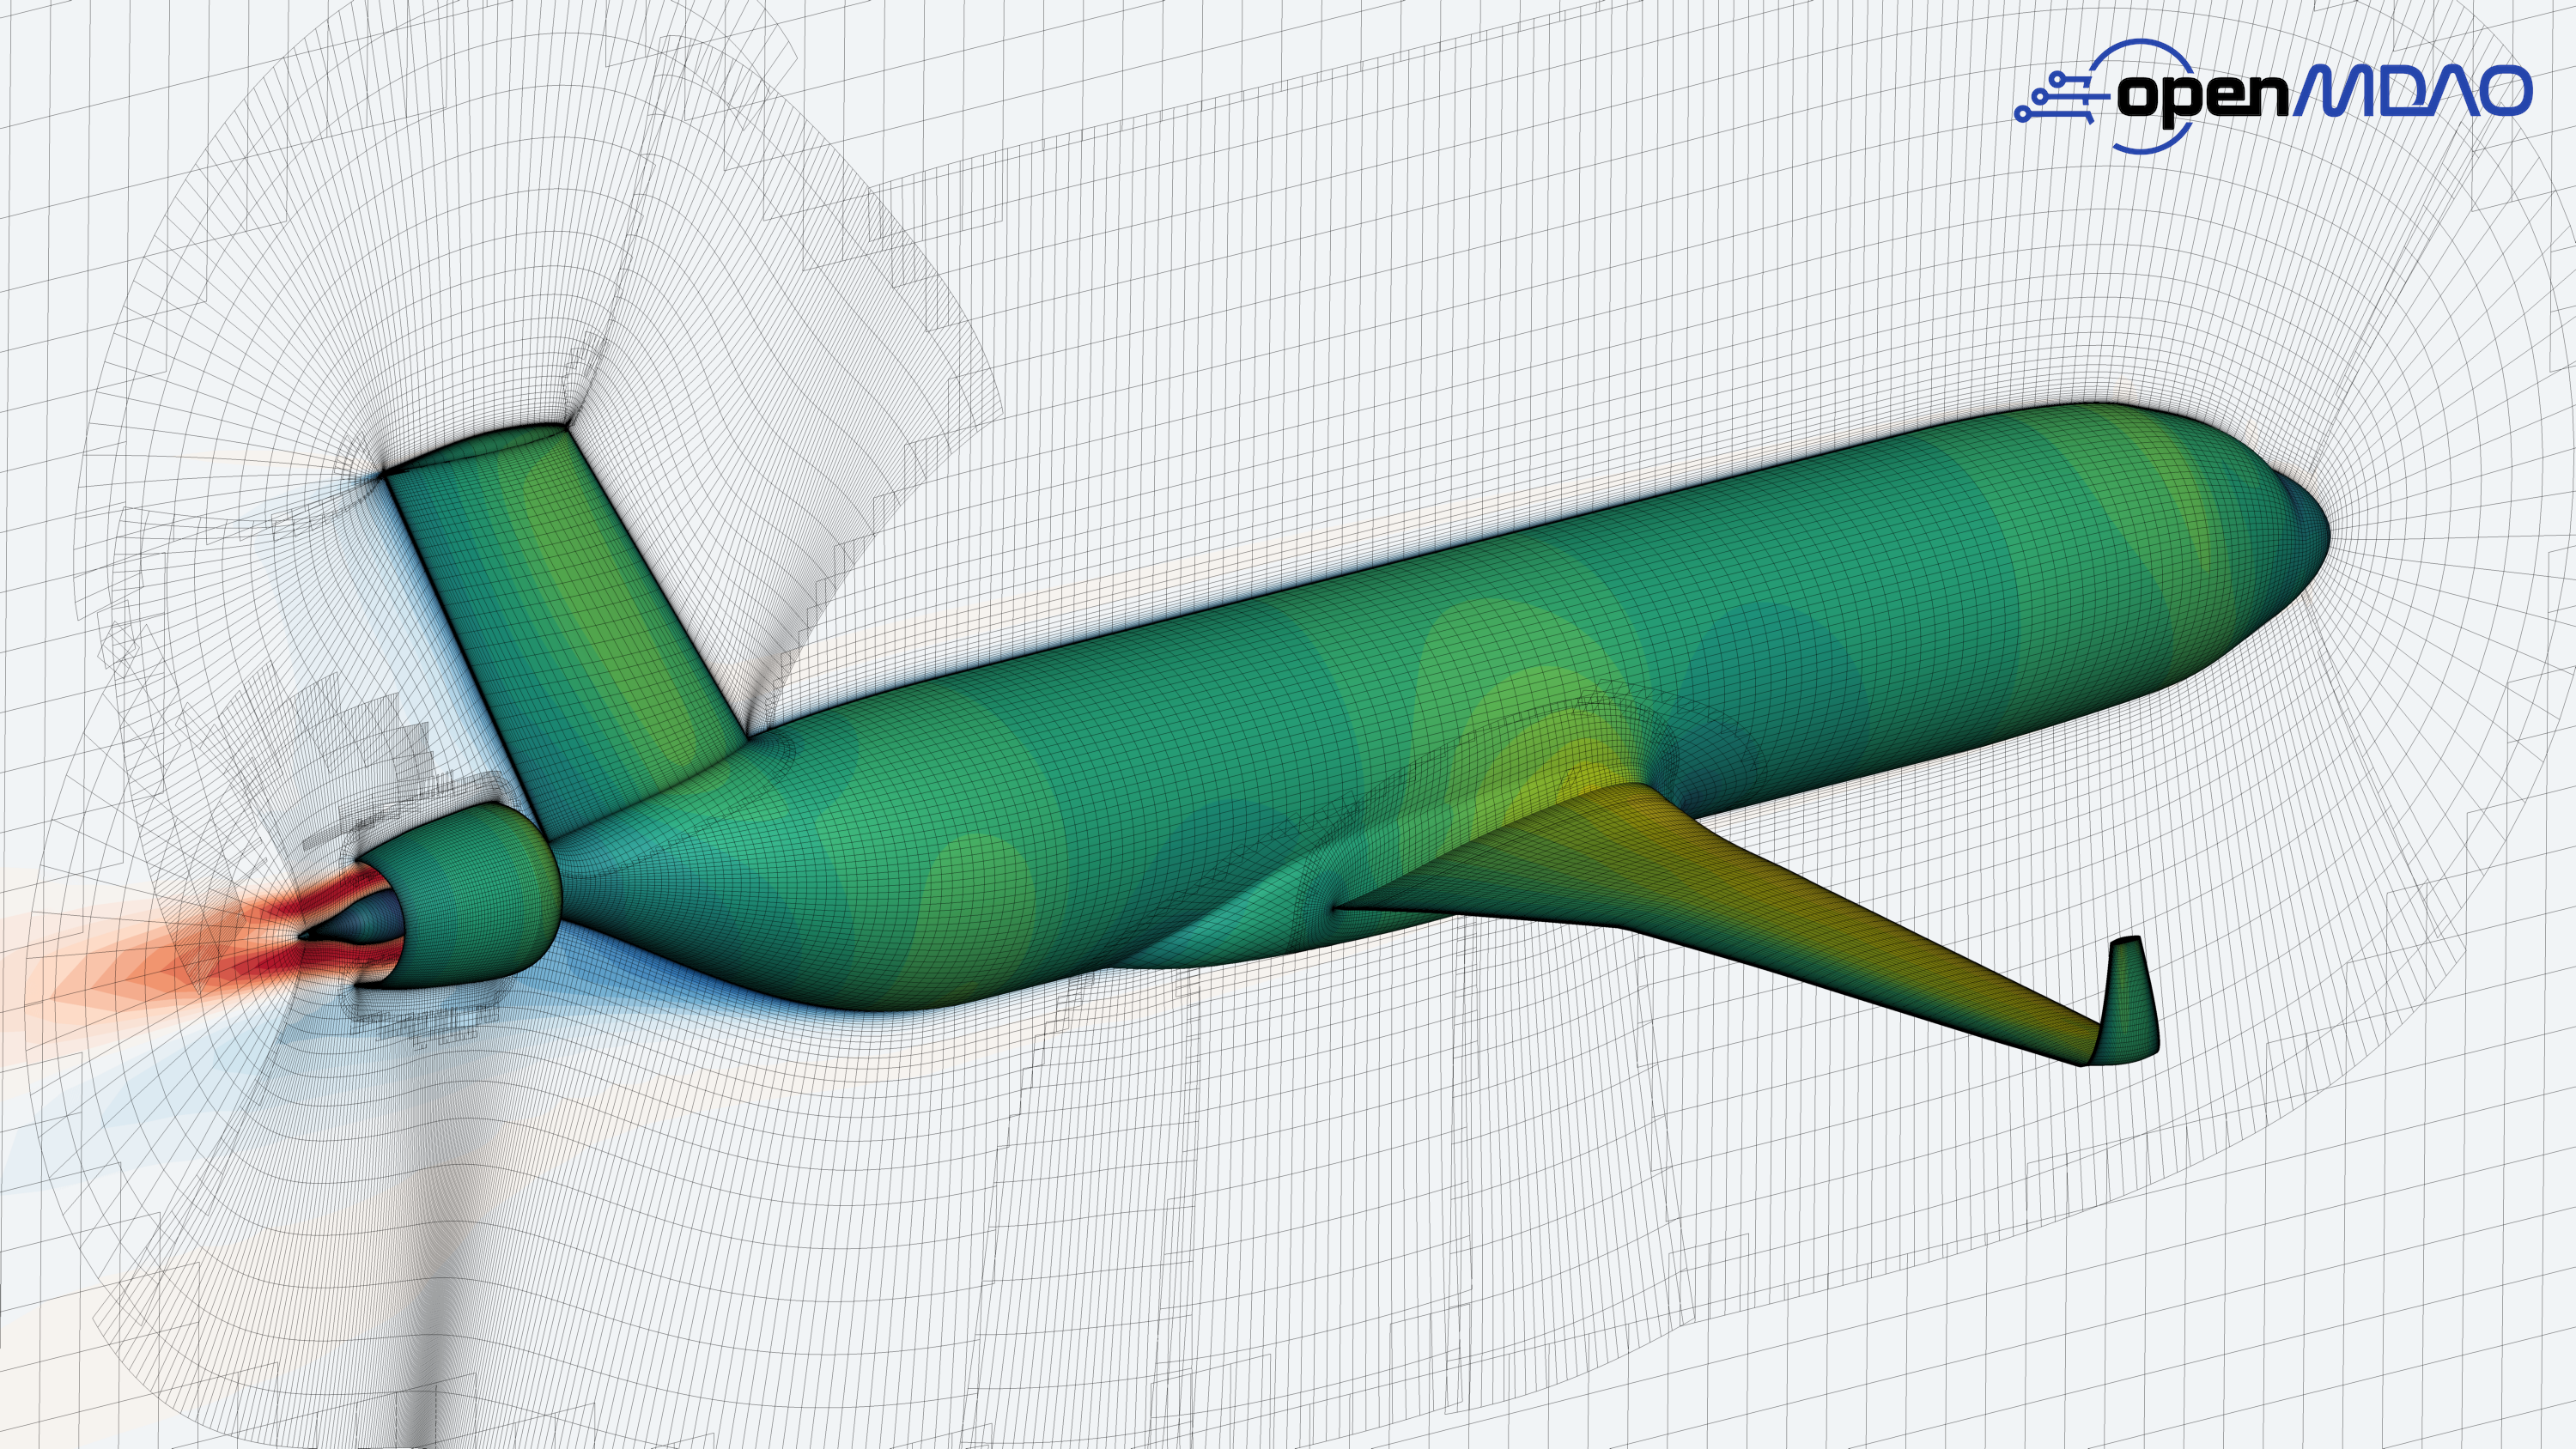
\includegraphics[
      width=0.8\columnwidth
    ]{figures/openmdao_slide.png}
  }

  (Multi-Disciplinary Analysis and Optimization)

  \vspace{\baselineskip}

  \begin{itemize}
  \item[--] Python OOP
  \item[--] Industry standard
  \end{itemize}
\end{frame}

\begin{frame}{OpenMDAO class structure}
  \center{
    \phantom{(These are the parts we care about)}
    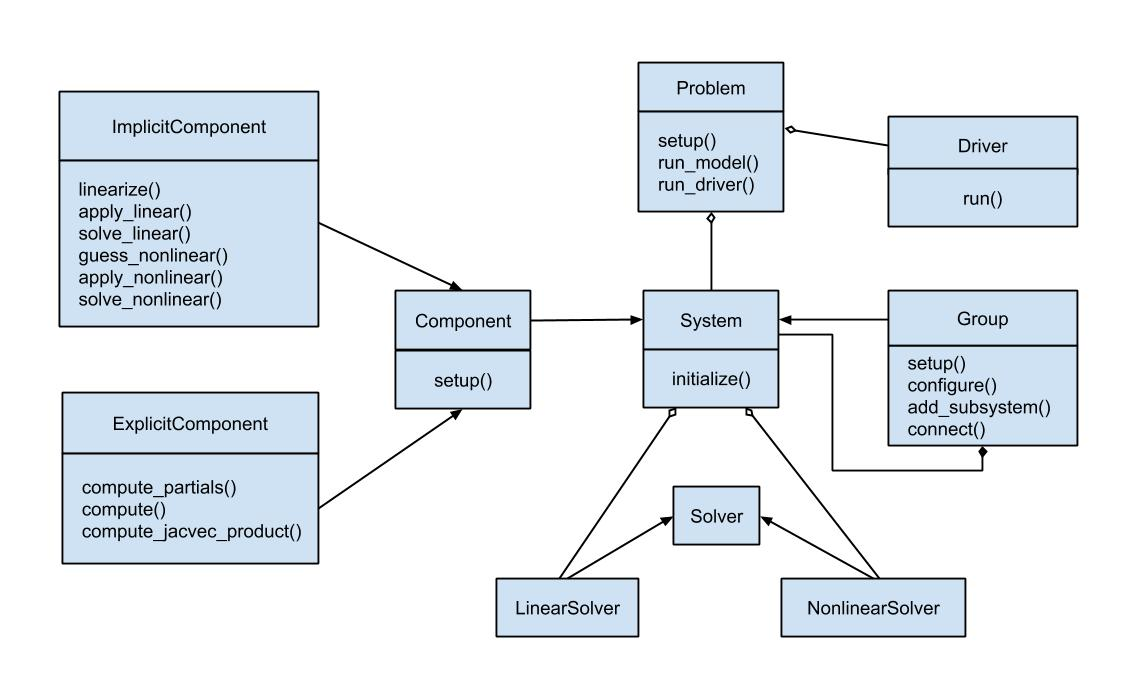
\includegraphics[
      width=\columnwidth
    ]{figures/openmdao_class_structure.jpg}
  }
\end{frame}

\begin{frame}{OpenMDAO class structure}
  (These are the parts we care about)

  \center{
    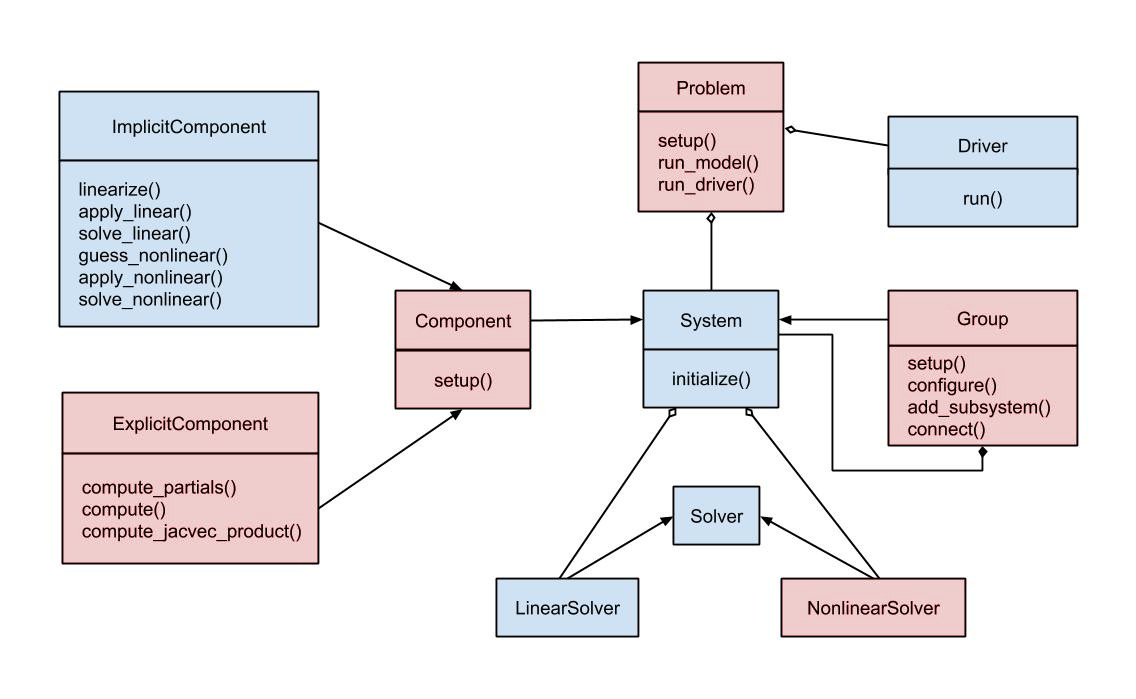
\includegraphics[
      width=\columnwidth
    ]{figures/openmdao_class_structure_highlight.jpg}
  }
\end{frame}

\begin{frame}{OpenMDAO class structure}
  This assembles into a tree-like structure with

  \begin{itemize}
  \item[--] \lstinline{Problem}'s internal Model class at root,
  \item[--] \lstinline{Group} intances as branching nodes, and
  \item[--] \lstinline{Component} instances as leaves:
  \end{itemize}

  \vspace{\baselineskip}

  \center{
    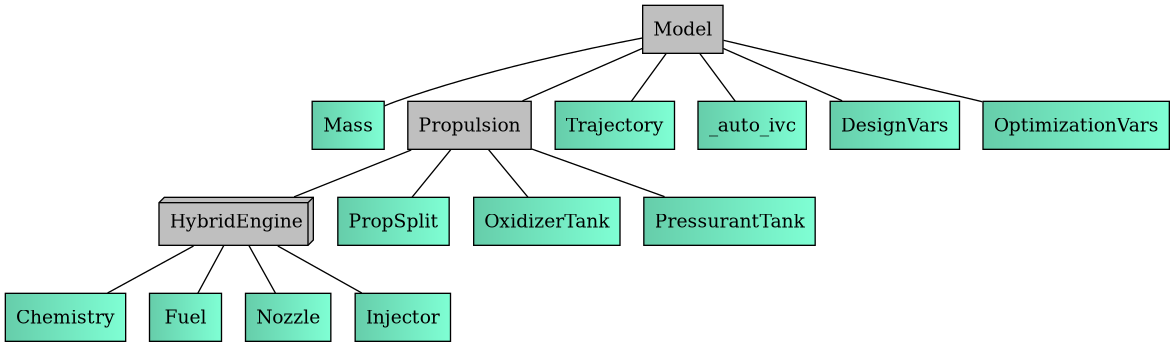
\includegraphics[width=\columnwidth]{figures/rocket_tree.png}
  }
\end{frame}

\begin{frame}{OpenMDAO class structure}
  \emph{Readability:} What does the code for this look like?

  \pause
  \vspace{\baselineskip}

  In the following: \emph{OpenMDAO by example}
\end{frame}


\subsection{Components}
\begin{frame}[fragile]{OpenMDAO Component class}
  \begin{lstlisting}[basicstyle=\ttfamily\tiny]
  # Components are the individual assembly units
  # that are a responsibility of a single working group

  class FooComponent(ExplicitComponent):

      def initialize(self):
          self.options.declare("foo", default=10.0, types=float)

      def setup(self):
          self.add_input("bar",  val=1.0, units="m")
          self.add_input("baz",  val=1.0, units="m")

          self.add_output("xyz", val=2.0, units="m")
          self.add_output("ijk", val=2.0, units="m")

      def setup_partials(self):
          self.declare_partials("*", "*", method="cs")

      def compute(self, inputs, outputs):
          bar = inputs["bar"]

          foo = self.options["foo"]

          baz = calc_baz(foo, bar)

          outputs["baz"] = baz
  \end{lstlisting}
\end{frame}

\begin{frame}[fragile]{OpenMDAO Component class}
  \begin{lstlisting}
  def initialize(self):
      # This is where you put immutable and
      # technical arguments of the class

      self.options.declare("foo", default=10.0,
                           types=float)
  \end{lstlisting}
\end{frame}

\begin{frame}[fragile]{OpenMDAO Component class}
  \begin{lstlisting}
  def setup(self):
      # This is where you define the way your part
      # interfaces to the rest of the assembly

      # Inputs: data that you need from the assembly
      self.add_input("bar",  val=1.0, units="m")
      self.add_input("baz",  val=1.0, units="m")

      # Outputs: data you provide to the assembly
      self.add_output("xyz", val=2.0, units="m")
      self.add_output("ijk", val=2.0, units="m")
  \end{lstlisting}
\end{frame}

\begin{frame}[fragile]{OpenMDAO Component class}
  \begin{lstlisting}
  def compute(self, inputs, outputs):
      # This is where your inputs
      # get mapped to your outputs

      # Collect inputs and options, ...
      bar = inputs["bar"]
      baz = inputs["baz"]
      foo = self.options["foo"]

      # ... perform calculations on them, ...
      xyz, ijk = calc_foo(foo, bar, baz)

      # ... and assign the results to the outputs
      outputs["xyz"] = xyz
      outputs["ijk"] = ijk
  \end{lstlisting}
\end{frame}


\subsection{Groups}
\begin{frame}[fragile]{OpenMDAO Group class}
  \begin{lstlisting}[basicstyle=\ttfamily\tiny]
  # Groups assemble and connect components together,
  # and have to deal with the flow of data between components

  class QuuxGroup(Group):

      def initialize(self):
          self.options.declare("foo", default=10.0, types=float)

      def setup(self):
          self.add_input("bar",  val=1.0, units="m")

          self.add_subsystem(
              "Foo",
              FooComponent(foo),
              promotes_inputs  = [("bar", "foo_bar")],
              promotes_outputs = [("xyz", "foo_xyz")],
          )

          self.add_subsystem(
              "Faz",
              FazComponent(foo),
              promotes_inputs  = [("bar", "faz_bar")],
              promotes_outputs = [("xyz", "faz_xyz")],
          )

          self.connect("Foo.ijk", "Faz.baz")
  \end{lstlisting}
\end{frame}

\begin{frame}[fragile]{OpenMDAO Group class}
  \begin{lstlisting}
  # Groups can promote inputs and outputs of their
  # components, in which case the promoted
  # input (output) becomes the input (ouptut)
  # of the whole group viewed as a component

  self.add_subsystem(
      "Foo",
      FooComponent(foo),
      promotes_inputs  = [("bar", "foo_bar")],
      promotes_outputs = [("xyz", "foo_xyz")],
      # . . . . . . . . . ^~~~~~~~~~~~~~~~~^
      # This tuple syntax instructs OpenMDAO
      # to rename inputs and outputs
      # to avoid naming clashes
  )
  \end{lstlisting}
\end{frame}

\begin{frame}[fragile]{OpenMDAO Group class}
  \begin{lstlisting}
  # Groups can connect inputs and outputs
  # of their components

  self.connect("Foo.ijk", "Faz.baz")

  # In the ideal case, inputs and outputs
  # are mapped cleanly without circular dependencies
  \end{lstlisting}
\end{frame}

\begin{frame}[fragile]{OpenMDAO Group class}
  \begin{lstlisting}
  # These connections can sometimes create
  # circular relations, which have to be
  # handled with nonlinear solvers

  self.nonlinear_solver
    = om.NewtonSolver(solve_subsystems=False)

  self.nonlinear_solver.options["maxiter"] = 30
  self.nonlinear_solver.options["rtol"]    = 1e-6
  self.nonlinear_solver.options["iprint"]  = 0

  self.nonlinear_solver.linesearch
    = om.ArmijoGoldsteinLS()

  self.linear_solver = om.DirectSolver()

  # This is an example of a very basic Newton's
  # method solver from our Propulsion group.
  # It is simple and efficient
  # under the right conditions
  \end{lstlisting}
\end{frame}


\subsection{Problems}
\begin{frame}[fragile]{OpenMDAO Problem class}
  A \lstinline{Problem} is a special kind of top-level \lstinline{Group}

  \vspace{\baselineskip}

  \begin{lstlisting}
  class HogeProblem(Problem):
      def __init__(self, foo, **kwargs):
          super().__init__(**kwargs)

          # A Problem models a top-level
          # Group or Component
          self.model = QuuxGroup(foo = foo)

          # It also contains a driver for any
          # non-linear optimization
          # happening internally
          self.driver = om.ScipyOptimizeDriver()
          self.driver.options["optimizer"] = "SLSQP"

  # Rest of the code can retrieve optimized values
  # after running the optimization driver
  hp = HogeProblem(foo)
  hp.run_driver()
  xyz_opt = hp.get_val("QuuxGroup.foo_xyz")[0]
  \end{lstlisting}
\end{frame}


\section{Rocket Assembly}
\begin{frame}{Rocket assembly, class structure}
  Reminder: OpenMDAO class structure
  \center{
    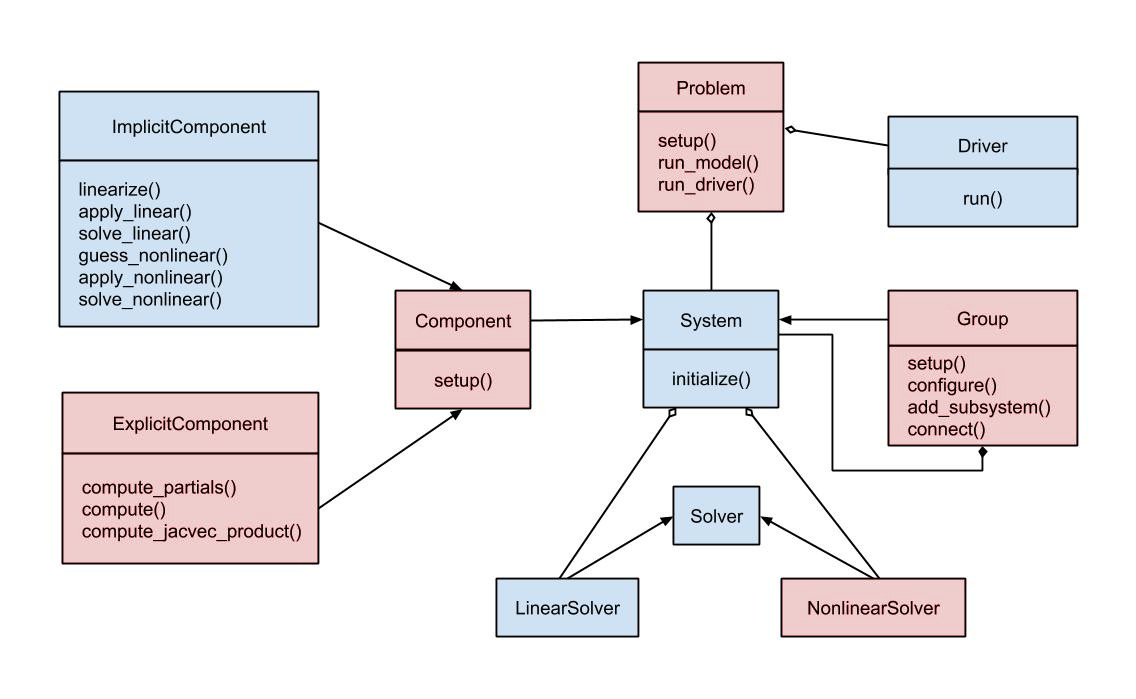
\includegraphics[
      width=\columnwidth
    ]{figures/openmdao_class_structure_highlight.jpg}
  }
\end{frame}

\begin{frame}{Hybrid rocket engine structure}
  Reminder: hybrid engine rocket structure
  \center{
    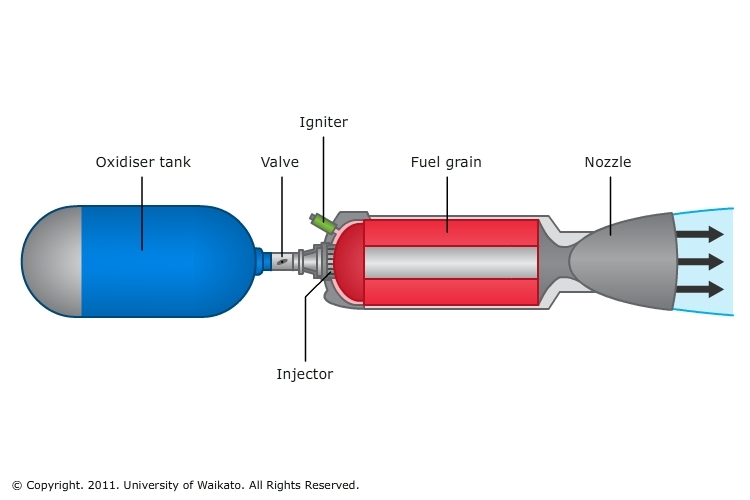
\includegraphics[width=\columnwidth]{figures/Hybrid-rocket-engine.jpg}
  }
\end{frame}

\begin{frame}{Rocket assembly, class structure}
  \centering
  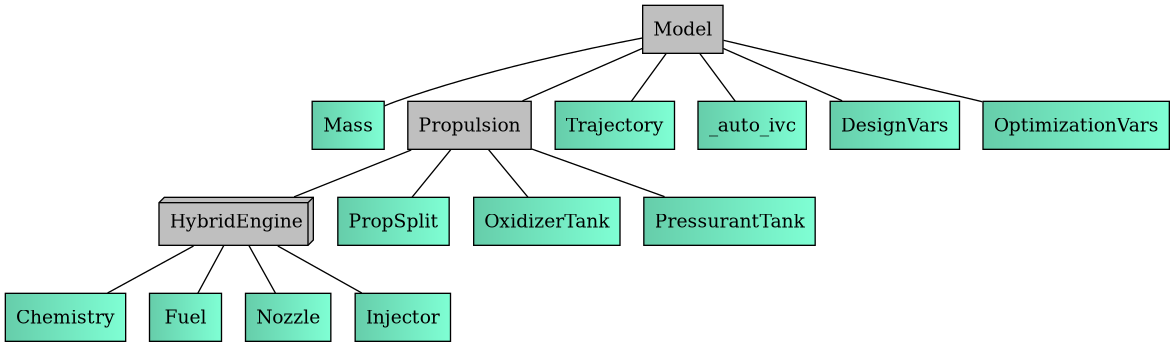
\includegraphics[width=\columnwidth]{figures/rocket_tree.png}
\end{frame}

\begin{frame}{Rocket assembly, data flow diagram}
  \centering
  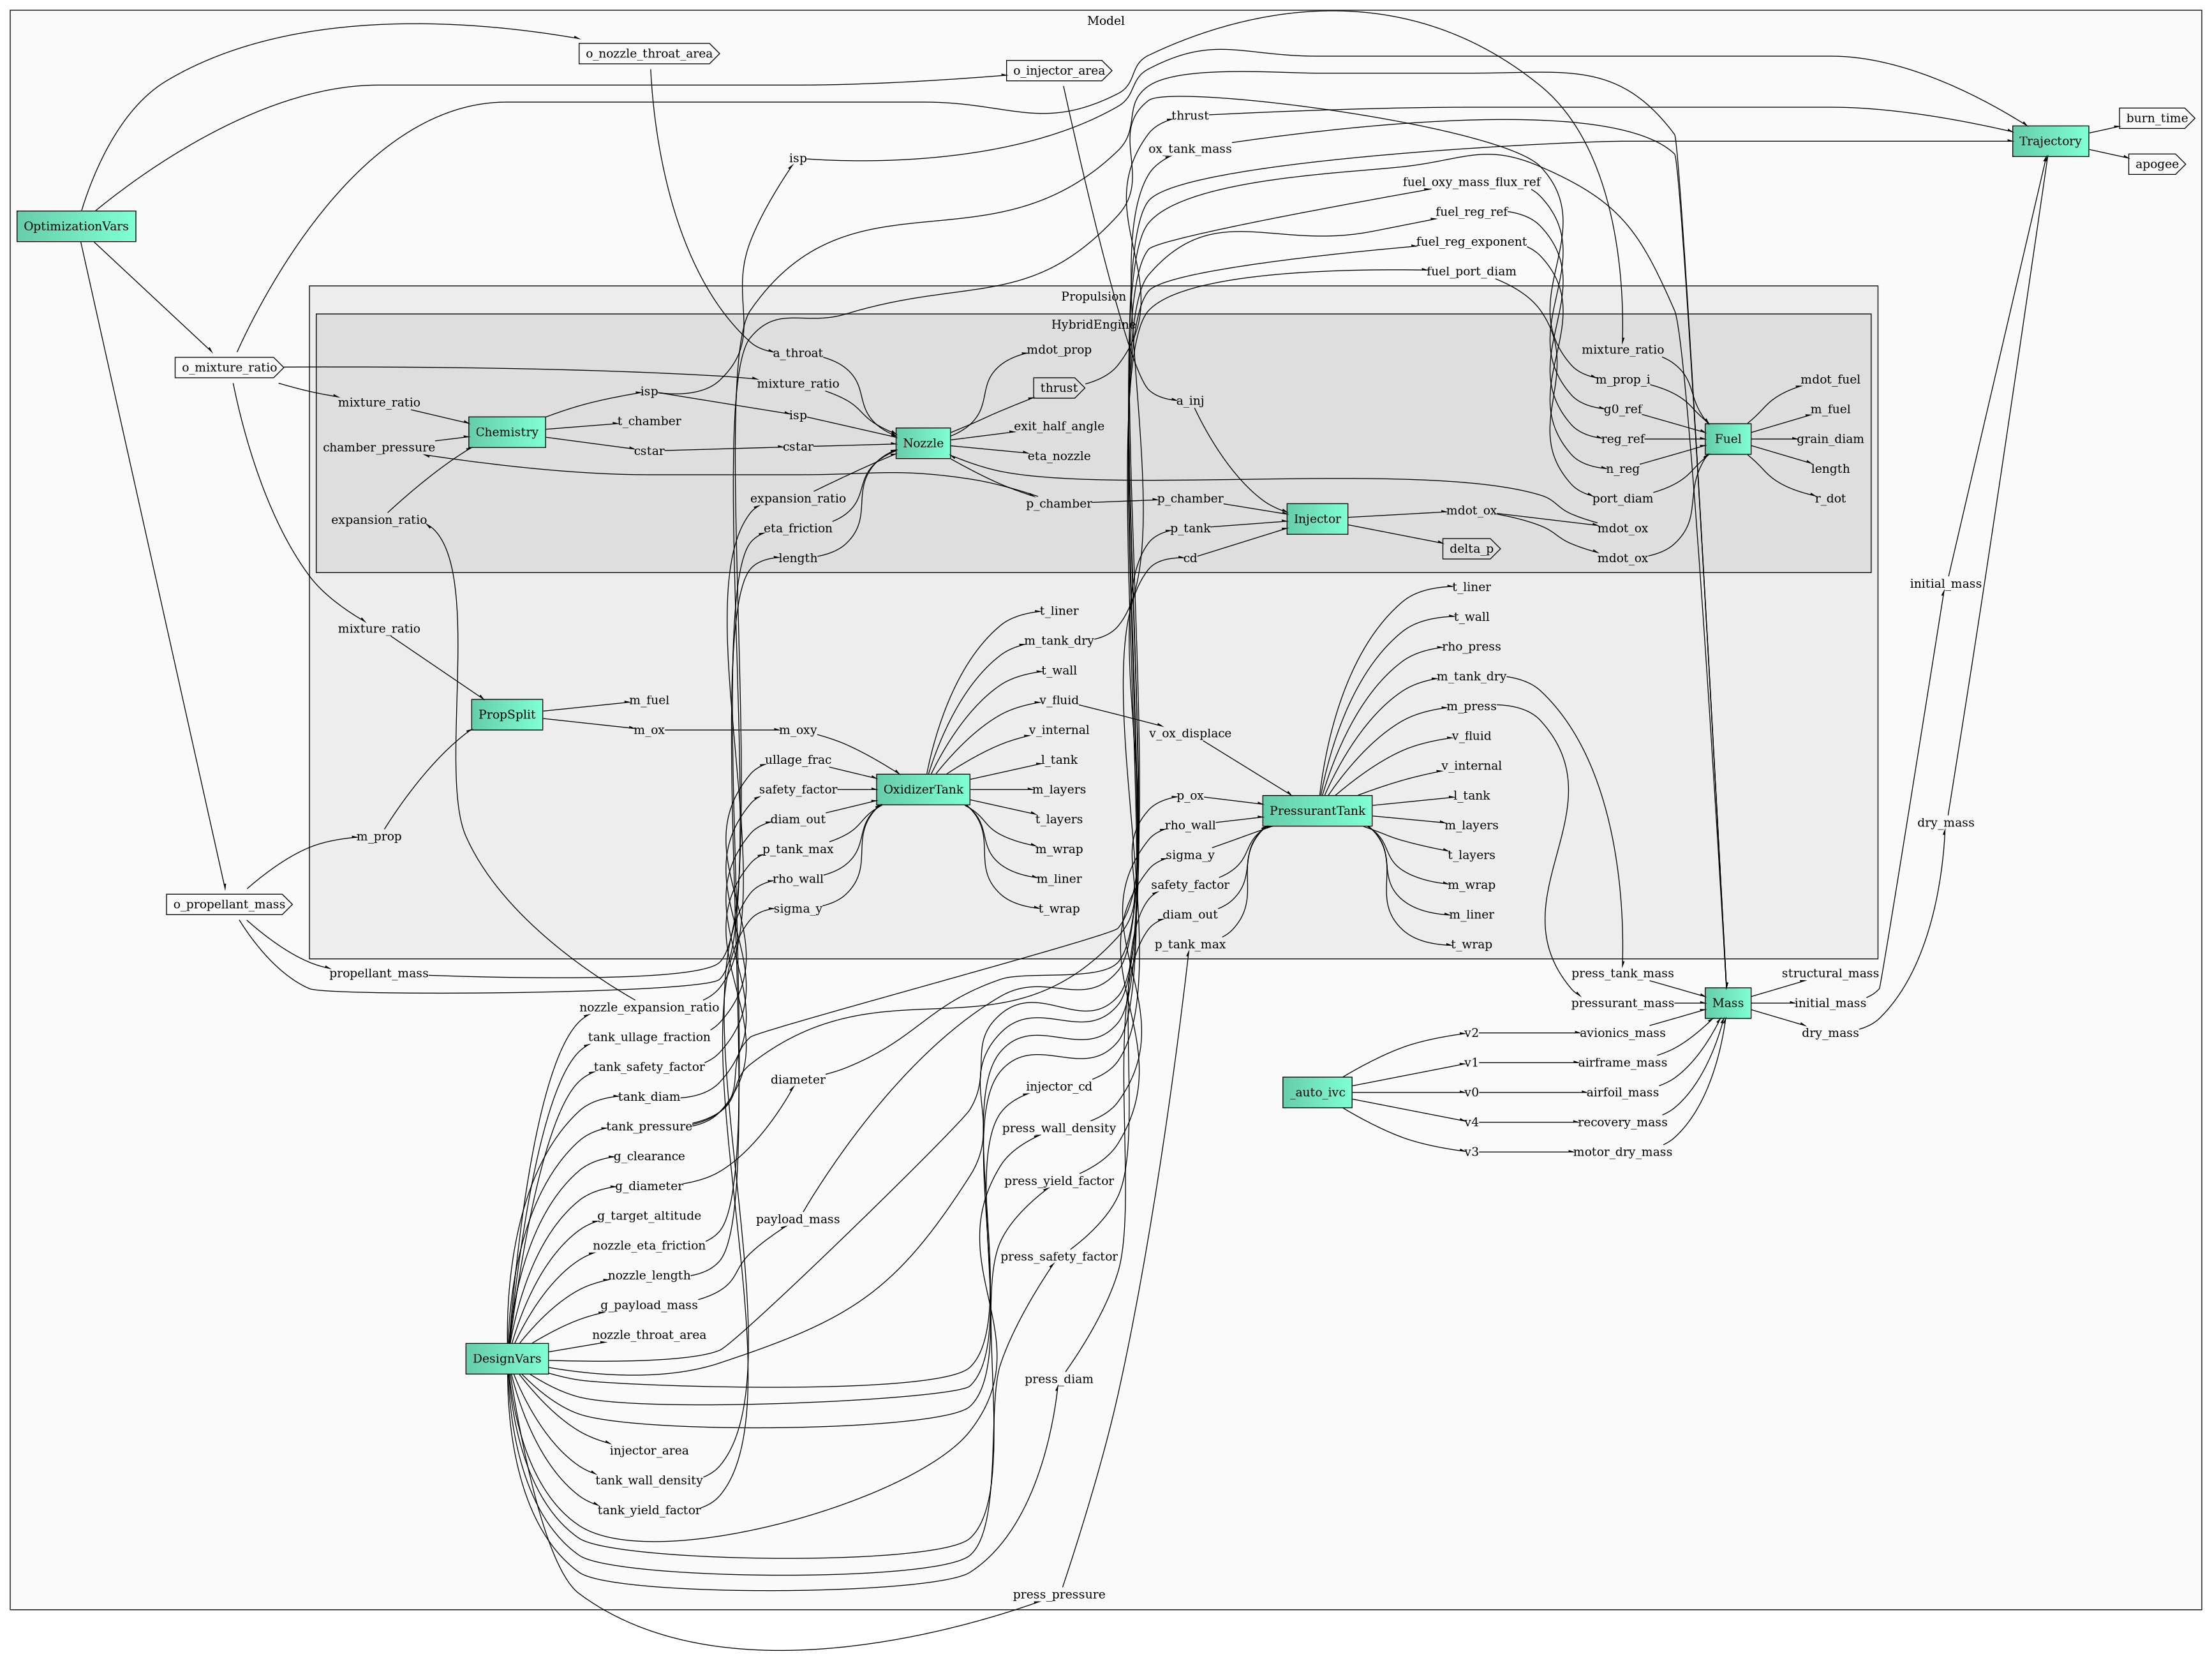
\includegraphics[width=\columnwidth]{figures/rocket_dataflow.png}
\end{frame}


\subsection{Hybrid Engine Nonlinearity}
\begin{frame}{Hybrid engine nonlinearity}
  The components of the \lstinline{HybridEngine} group form a closed loop:

  \vspace{\baselineskip}


  \begin{description}[align=right, leftmargin=*, widest=Chemistry]
  \item[Injector] Incompressible orifice plate flow:
    \begin{equation*}
      \dot{m}_\text{ox}
      = C_\text{d} A_\text{inj}
        \sqrt{2\rho_\text{ox} (P_\text{tank} - P_\text{c})}
    \end{equation*}
    {
      \tiny
      (Source:
      \url{https://en.wikipedia.org/wiki/Orifice\_plate\#Incompressible\_flow})
    }
  \item[Chemistry] Gibbs free energy equilibrium \\
    (solved internally by the CEA library):
    \begin{equation*}
      c^* = f_\text{CEA} (P_\text{c}, \mathrm{MR})
    \end{equation*}
  \item[Nozzle] Choked flow:
    \begin{equation*}
      P_\text{c}
      = \frac{\dot{m}_\text{prop} \cdot c^*}{A_\text{t}}
      = \frac{\dot{m}_\text{ox} \left(1 - \frac{1}{\mathrm{MR}}\right)c^*}
             {A_\text{t}}
    \end{equation*}
    {
      \tiny
      (Source: \url{https://en.wikipedia.org/wiki/Choked\_flow})
    }
  \end{description}
\end{frame}

\begin{frame}{Hybrid engine master equation}
  Substitute the injector and chemistry equations into the nozzle equation:

  \vspace{\baselineskip}

  \begin{equation*}
    P_\text{c}
    = \left[
        C_\mathrm{d}
        \frac{A_\text{inj}}{A_\text{t}}
        \left(1 + \frac{1}{\mathrm{MR}}\right)
      \right]
      \cdot \sqrt{2\rho_\text{ox} (P_\text{tank} - P_\text{c})}
      \cdot c^* (P_\text{c}, \mathrm{MR})
  \end{equation*}
\end{frame}

\begin{frame}{Hybrid engine solver}
  To solve this, use the residual function $R(P_\text{c}) = 0$:

  \begin{alignat*}{2}
    R(P_\text{c})
    = P_\text{c}
    - \bigg[ & \frac{A_\text{inj}}{A_\text{t}}
               C_\mathrm{d} \left(1 + \frac{1}{\mathrm{MR}}\right) \\
             & \cdot \sqrt{2\rho_\text{ox} (P_\text{tank} - P_\text{c})}
               \cdot c^* (P_\text{c}, \mathrm{MR}) \bigg] = 0
  \end{alignat*}

  OpenMDAO's \lstinline{NewtonSolver} solves $R(P_\text{c})=0$ using an initial
  guess and tangent lines:

  \begin{equation*}
    P_\text{c}^{(k+1)}
    = P_\text{c}^{(k)}
    - \frac{R(P_\text{c}^{(k)})}{\mathrm{d} R / \mathrm{d} P_\text{c}}
  \end{equation*}

  This usually converges in $\mathcal O(10)$ steps
\end{frame}


\section{Program Layout}
\begin{frame}{Rocket assembly, program structure}
  \centering
  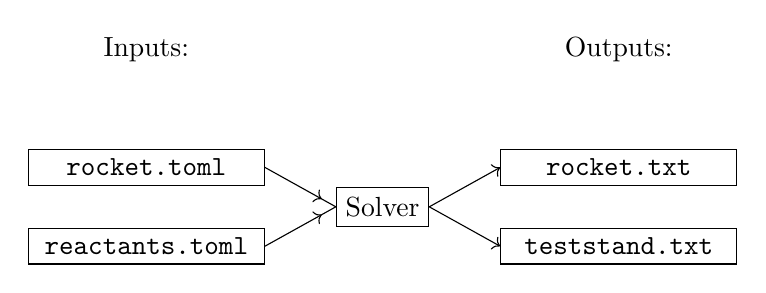
\begin{tikzpicture}
  \node[draw] (prog) at (0, 0) {Solver};

  \node[rectangle,       minimum width=3cm] (label1)  at (-3,  2  ) {Inputs:};
  \node[rectangle, draw, minimum width=3cm] (input1)  at (-3,  0.5) {\texttt{rocket.toml}};
  \node[rectangle, draw, minimum width=3cm] (input2)  at (-3, -0.5) {\texttt{reactants.toml}};

  \node[rectangle,       minimum width=3cm] (label2)  at (3,   2  ) {Outputs:};
  \node[rectangle, draw, minimum width=3cm] (output1) at ( 3,  0.5) {\texttt{rocket.txt}};
  \node[rectangle, draw, minimum width=3cm] (output2) at ( 3, -0.5) {\texttt{teststand.txt}};

  \draw[->-=.8] (input1.east) -- (prog.west);
  \draw[->-=.8] (input2.east) -- (prog.west);

  \draw[->] (prog.east) -- (output1.west);
  \draw[->] (prog.east) -- (output2.west);
  \end{tikzpicture}
\end{frame}

\begin{frame}[fragile]{Program inputs}
  The input files are configs in human-readable format:

  \vspace{\baselineskip}

  \begin{lstlisting}[language=TOML, basicstyle=\ttfamily\tiny]
  [global]
  payload_mass_kg         = 1.0
  target_altitude_m       = 3000.0
  diameter_m              = 0.12
  clearance_m             = 0.0

  [oxidizer_tank]
  pressure_bar            = 70.0
  diam_m                  = 0.12
  safety_factor           = 2.0
  ullage_fraction         = 0.1
  yield_factor_pa         = 2.76e8
  wall_density_kgm3       = 2700.0

  [pressurizer_tank]
  pressure_bar            = 200.0
  diam_m                  = 0.12
  safety_factor           = 2.0
  yield_factor_pa         = 2.76e8
  wall_density_kgm3       = 2700.0

  [injector]
  area_m2                 = 4.5e-5
  cd                      = 0.7
  .
  .
  .
  \end{lstlisting}
\end{frame}

\begin{frame}[fragile]{Program outputs}
  The output files are text printouts of OpenMDAO structure:

  \vspace{\baselineskip}

  \begin{minipage}{\textwidth}
  \begin{lstlisting}[
    language   = Fortran,
    basicstyle = \ttfamily\tiny,
    breaklines = false,
    columns    = fullflexible,
    keepspaces
  ]
  75 Explicit Output(s) in 'model'

  varname                   val                   units      prom_name
  ------------------------  --------------------  ---------  ---------------------------------
  DesignVars
    g_payload_mass          [1.]                  kg         DesignVars.g_payload_mass
    g_target_altitude       [3000.]               m          DesignVars.g_target_altitude
    tank_pressure           [70.]                 bar        DesignVars.tank_pressure
    tank_diam               [0.12]                m          DesignVars.tank_diam
    tank_safety_factor      [2.]                  None       DesignVars.tank_safety_factor
    .
    .
    .

  Propulsion
    PropSplit
      m_ox                  [1.54084888]          kg         Propulsion.PropSplit.m_ox
      m_fuel                [0.16938875]          kg         Propulsion.PropSplit.m_fuel
    OxidizerTank
      t_wall                [0.00147395]          m          Propulsion.tank_wall_thickness
      t_liner               [0.001]               m          Propulsion.tank_liner_thickness
      t_wrap                [0.00047395]          m          Propulsion.tank_wrap_thickness
      m_liner               [0.17283683]          kg         Propulsion.OxidizerTank.m_liner
      m_wrap                [0.04801895]          kg         Propulsion.OxidizerTank.m_wrap
      .
      .
      .
  \end{lstlisting}
  \end{minipage}
\end{frame}


\subsection{Modules}
\begin{frame}[fragile]{Rocket assembly, module structure}
  \begin{columns}
    \begin{column}{0.30\textwidth}
      \begin{verbatim}
solver.py
inputs/
└── ...
outputs/
└── ...
modules/
├── BEARS_Atmo
├── BEARS_Chem
├── BEARS_Materials
├── BEARS_Rocket
└── Config
      \end{verbatim}
    \end{column}
    \hfill
    \begin{column}{0.50\textwidth}
      \justifying

      The program is laid out in a number of modules according to their purpose

      \vspace{\baselineskip}

      Most \lstinline{compute()} functions carry out their computations in a few
      lines, but some computations are too long or require external libraries
      and have been offloaded to separate modules
    \end{column}
  \end{columns}
\end{frame}

\begin{frame}{Rocket assembly, modules}
  \begin{description}
  \item[\texttt{BEARS\_Rocket}] Core logic with the OpenMDAO model
    \pause
  \item[\texttt{BEARS\_Atmo}] Atmospheric model, offloaded to
    \lstinline{ISACALC}
    \pause
  \item[\texttt{BEARS\_Chem}] Reaction chemistry, offloaded to
    \lstinline{RocketCEA}
    \pause
  \item[\texttt{BEARS\_Materials}] Tank sizing and material calculations
    \pause
  \item[\texttt{Config}] Config loader technical module
  \end{description}

  \pause
  \vspace{\baselineskip}
  \justifying

  (The \lstinline{BEARS_*} prefix is omitted for \lstinline{Config} since it
  contains no meaningful physics)

  \vspace{\baselineskip}

  TODO: \lstinline{BEARS_Materials} possibly inconsistent/counterintuitive, it
  contains tank sizing logic and not just material properties
\end{frame}

\begin{frame}[fragile]{Rocket assembly, core module}
  \begin{columns}
    \begin{column}{0.30\textwidth}
      \begin{footnotesize}
      \begin{verbatim}
modules/BEARS_Rocket/
├── checks.py
├── comp_chem.py
├── comp_fuel.py
├── comp_injector.py
├── comp_mass.py
├── comp_nozzle.py
├── comp_split.py
├── comp_tank_oxy.py
├── comp_tank_press.py
├── comp_tank.py
├── comp_traj.py
├── group_engine.py
├── group_prop.py
├── group_rocket.py
├── group_teststand.py
├── prob_rocket.py
└── prob_teststand.py
      \end{verbatim}
      \end{footnotesize}
    \end{column}
    \hfill
    \begin{column}{0.50\textwidth}
      \justifying

      The core module is laid out in one-class-per-file structure following the
      OpenMDAO class layout

      \pause
      \vspace{\baselineskip}

      TODO: trajectory component is somewhat large and can be offloaded to a
      dedicated module
    \end{column}
  \end{columns}
\end{frame}


\subsection{Checks Module}
\begin{frame}[fragile]{Checks module}
  \textbf{\texttt{checks.py}:}

  \vspace{\baselineskip}

  Keeping with the goal of extensibility: dedicated module for team members to
  implement post-run sanity checks

  \vspace{\baselineskip}

  \begin{lstlisting}
  class CheckResult(NamedTuple):
      severity : Literal["error", "warning"]
      message  : str

  CheckFn
    = Callable[[Problem], tuple[CheckResult, ...]]
  \end{lstlisting}
\end{frame}

\begin{frame}[fragile]{Check functions}
  \begin{lstlisting}[basicstyle=\ttfamily\tiny]
  # Example: launch TWR sanity check

  def check_liftoff_twr(prob: Problem) -> tuple[CheckResult, ...]:
      issues: list[CheckResult] = []

      thr = prob.get_val("Propulsion.prop_thrust", units="N")[0]
      mi  = prob.get_val("Mass.initial_mass",      units="kg")[0]

      twr = thr / (mi * g)

      if twr < 1.0:
          issues.append(CheckResult(
              "error",
              f"Liftoff TWR below 1.0 ({twr:.3f})"
          ))
      elif twr < 1.3:
          issues.append(CheckResult(
              "warning",
              f"Liftoff TWR is low ({twr:.3f})"
          ))

      return tuple(issues)
  \end{lstlisting}
\end{frame}


\section{Next steps}
\begin{frame}{Next steps}
  We consider the current state of the program mostly production-ready with few
  exceptions

  \vspace{\baselineskip}

  \begin{itemize}
  \item[--] \textbf{Get subgroup members to start editing system components}
  \item[--] Drag calculations are long and can be offloaded to a dedicated
    module
  \item[--] Materials module rewrite with Rishabh's new code
  \item[--] Lots of small details need fixing in individual modules
  \item[--] Better naming?
  \end{itemize}
\end{frame}

\begin{frame}{Calculations people}
  \begin{figure}
  \captionsetup{labelformat=empty}
  \begin{minipage}{0.3\linewidth}
    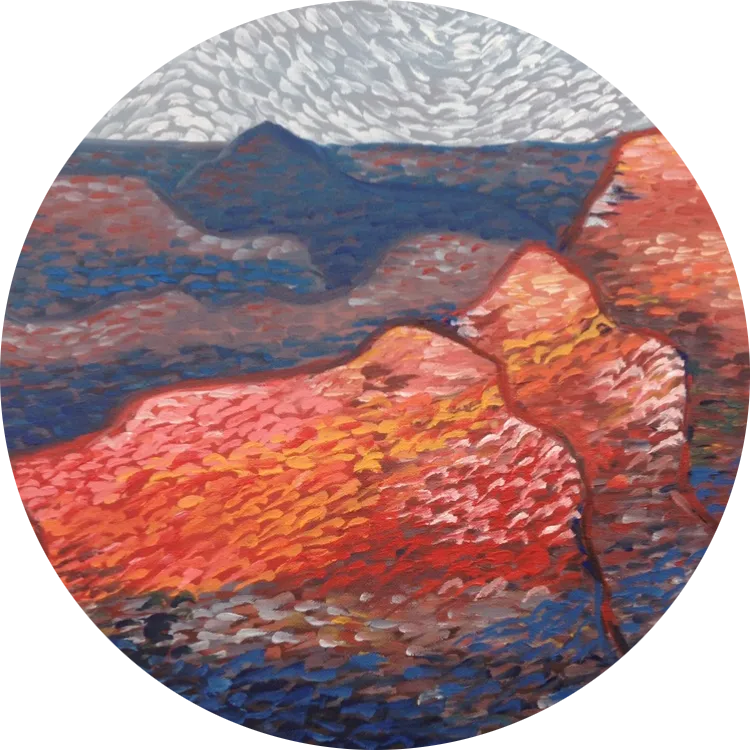
\includegraphics[width=\textwidth]{figures/andrii-avi.png}
    \caption{Andrii}
  \end{minipage}
  \hfill
  \begin{minipage}{0.3\linewidth}
    
\includegraphics[width=\textwidth]{figures/noa-avi.png}
    \caption{Noa}
  \end{minipage}
  \hfill
  \begin{minipage}{0.3\linewidth}
    
\includegraphics[width=\textwidth]{figures/sophia-avi.png}
    \caption{Sophia}
  \end{minipage}
  \end{figure}
\end{frame}


\begin{frame}{Next steps}
  \justifying

  Once the current calculations program is fleshed out, we will proceed with
  merging the solver with BEARS' flight sim program \lstinline{rocketpal} on a
  new branch, while master with the current structure remains for support

  \center{
    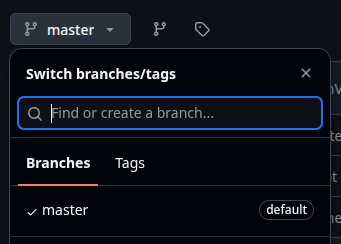
\includegraphics[width=0.5\columnwidth]{figures/branches.png}
  }
\end{frame}

\begin{frame}{Integration plan}
  \centering
  \resizebox{\textwidth}{!}{
    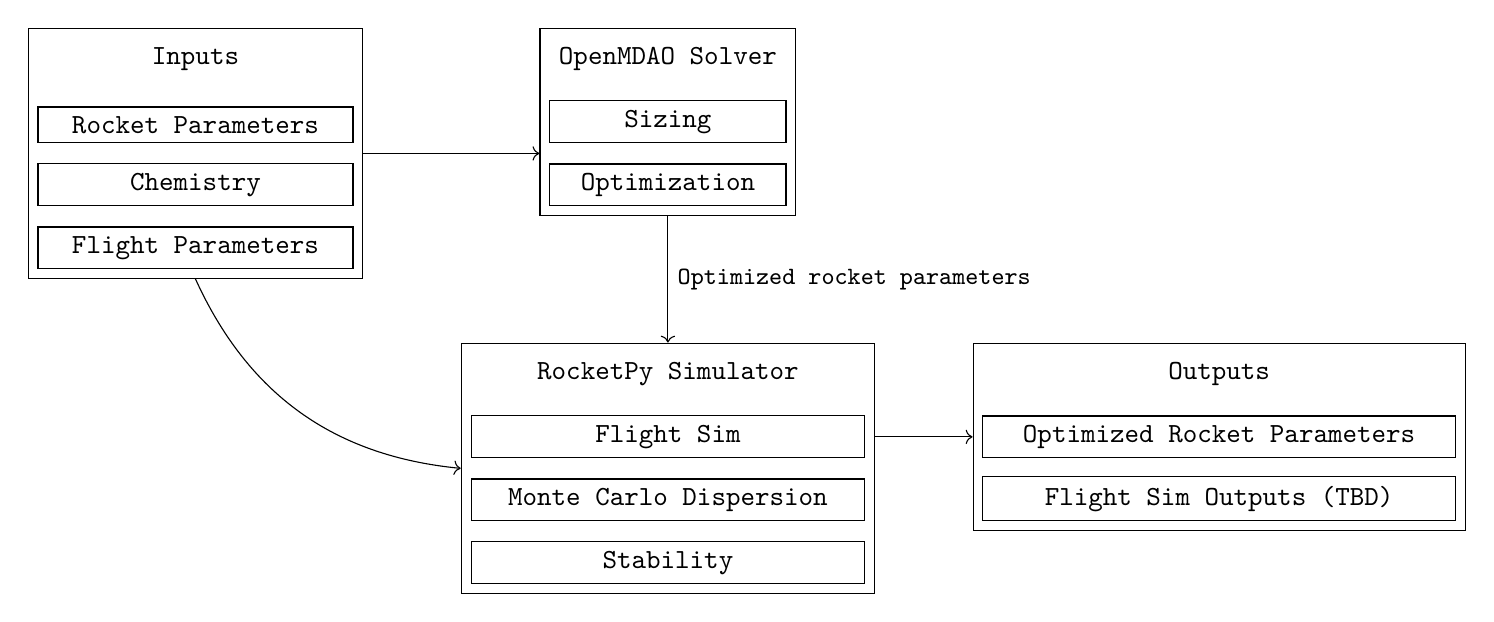
\begin{tikzpicture}[
      %transform canvas = {scale=0.6},
      node distance    = 8mm,
      s/.style         = {font=\ttfamily}
    ]
    % Inputs
    \node (inp) at (-6, 0) [s] {Inputs};

    \node (inp1) [
      s, draw, below=of inp.south,  anchor=south, minimum width=4cm
    ] {Rocket Parameters};

    \node (inp2) [
      s, draw, below=of inp1.south,  anchor=south, minimum width=4cm
    ] {Chemistry};

    \node (inp3) [
      s, draw, below=of inp2.south,  anchor=south, minimum width=4cm
    ] {Flight Parameters};

    \node[draw, fit={(inp) (inp1) (inp2) (inp3)}] (inpt) {};

    % Solver
    \node (solv) at (0, 0) [s] {OpenMDAO Solver};

    \node (solv1) [
      s, draw, below=of solv.south,  anchor=south, minimum width=3cm
    ] {Sizing};

    \node (solv2) [
      s, draw, below=of solv1.south, anchor=south, minimum width=3cm
    ] {Optimization};

    \node[draw, fit={(solv) (solv1) (solv2)}] (solvt) {};

    % Simulator
    \node (sim) at (0, -4) [s] {RocketPy Simulator};

    \node (sim1) [
      s, draw, below=of sim.south,  anchor=south, minimum width=5cm
    ] {Flight Sim};

    \node (sim2) [
      s, draw, below=of sim1.south, anchor=south, minimum width=5cm
    ] {Monte Carlo Dispersion};

    \node (sim3) [
      s, draw, below=of sim2.south, anchor=south, minimum width=5cm
    ] {Stability};

    \node[draw, fit={(sim) (sim1) (sim2) (sim3)}] (simt) {};

    % Outputs
    \node (out) at (7, -4) [s] {Outputs};

    \node (out1) [
      s, draw, below=of out.south,  anchor=south, minimum width=6cm
    ] {Optimized Rocket Parameters};

    \node (out2) [
      s, draw, below=of out1.south, anchor=south, minimum width=6cm
    ] {Flight Sim Outputs (TBD)};

    \node[draw, fit={(out) (out1) (out2)}] (outt) {};

    % Connections
    \draw[->] (inpt) -- (inpt.east -| solvt.west);
    \draw[->] (inpt.south) to [bend right] (simt.west);

    \draw[->] (solvt) -- (simt) node[
      style={font=\ttfamily\small}, midway, right
    ] {Optimized rocket parameters};

    \draw[->] (simt.east |- outt.west) -- (outt.west);
    \end{tikzpicture}
  }
\end{frame}


\end{document}
